\subsection{Structure of a Remixing System} 
I plan to study the sociotechnical architecture of the Scratch Online Community by examining its following structural attributes (Figure~\ref{fig:structure}):
1) granularity of the remixable components, 
2) modularity of the remixable components, 
3) decomposability of finished projects, 
4) attributability mechanisms, and 
5) openness to remix across systems.

In this proposal I briefly define each structural attribute using one or two examples, and I explain how I am planning to go about studying it.
I plan to analyze these structural properties of the system using varied approaches including:
1) case studies that give a rich description of various scenarios that explain the influence of each attribute,
2) analyses of the data corpus to understand the frequency of the scenarios and the relationships among the structural attributes,
3) natural design experiments to study the effect of varying some structural dimensions.

\begin{figure} 
\centering
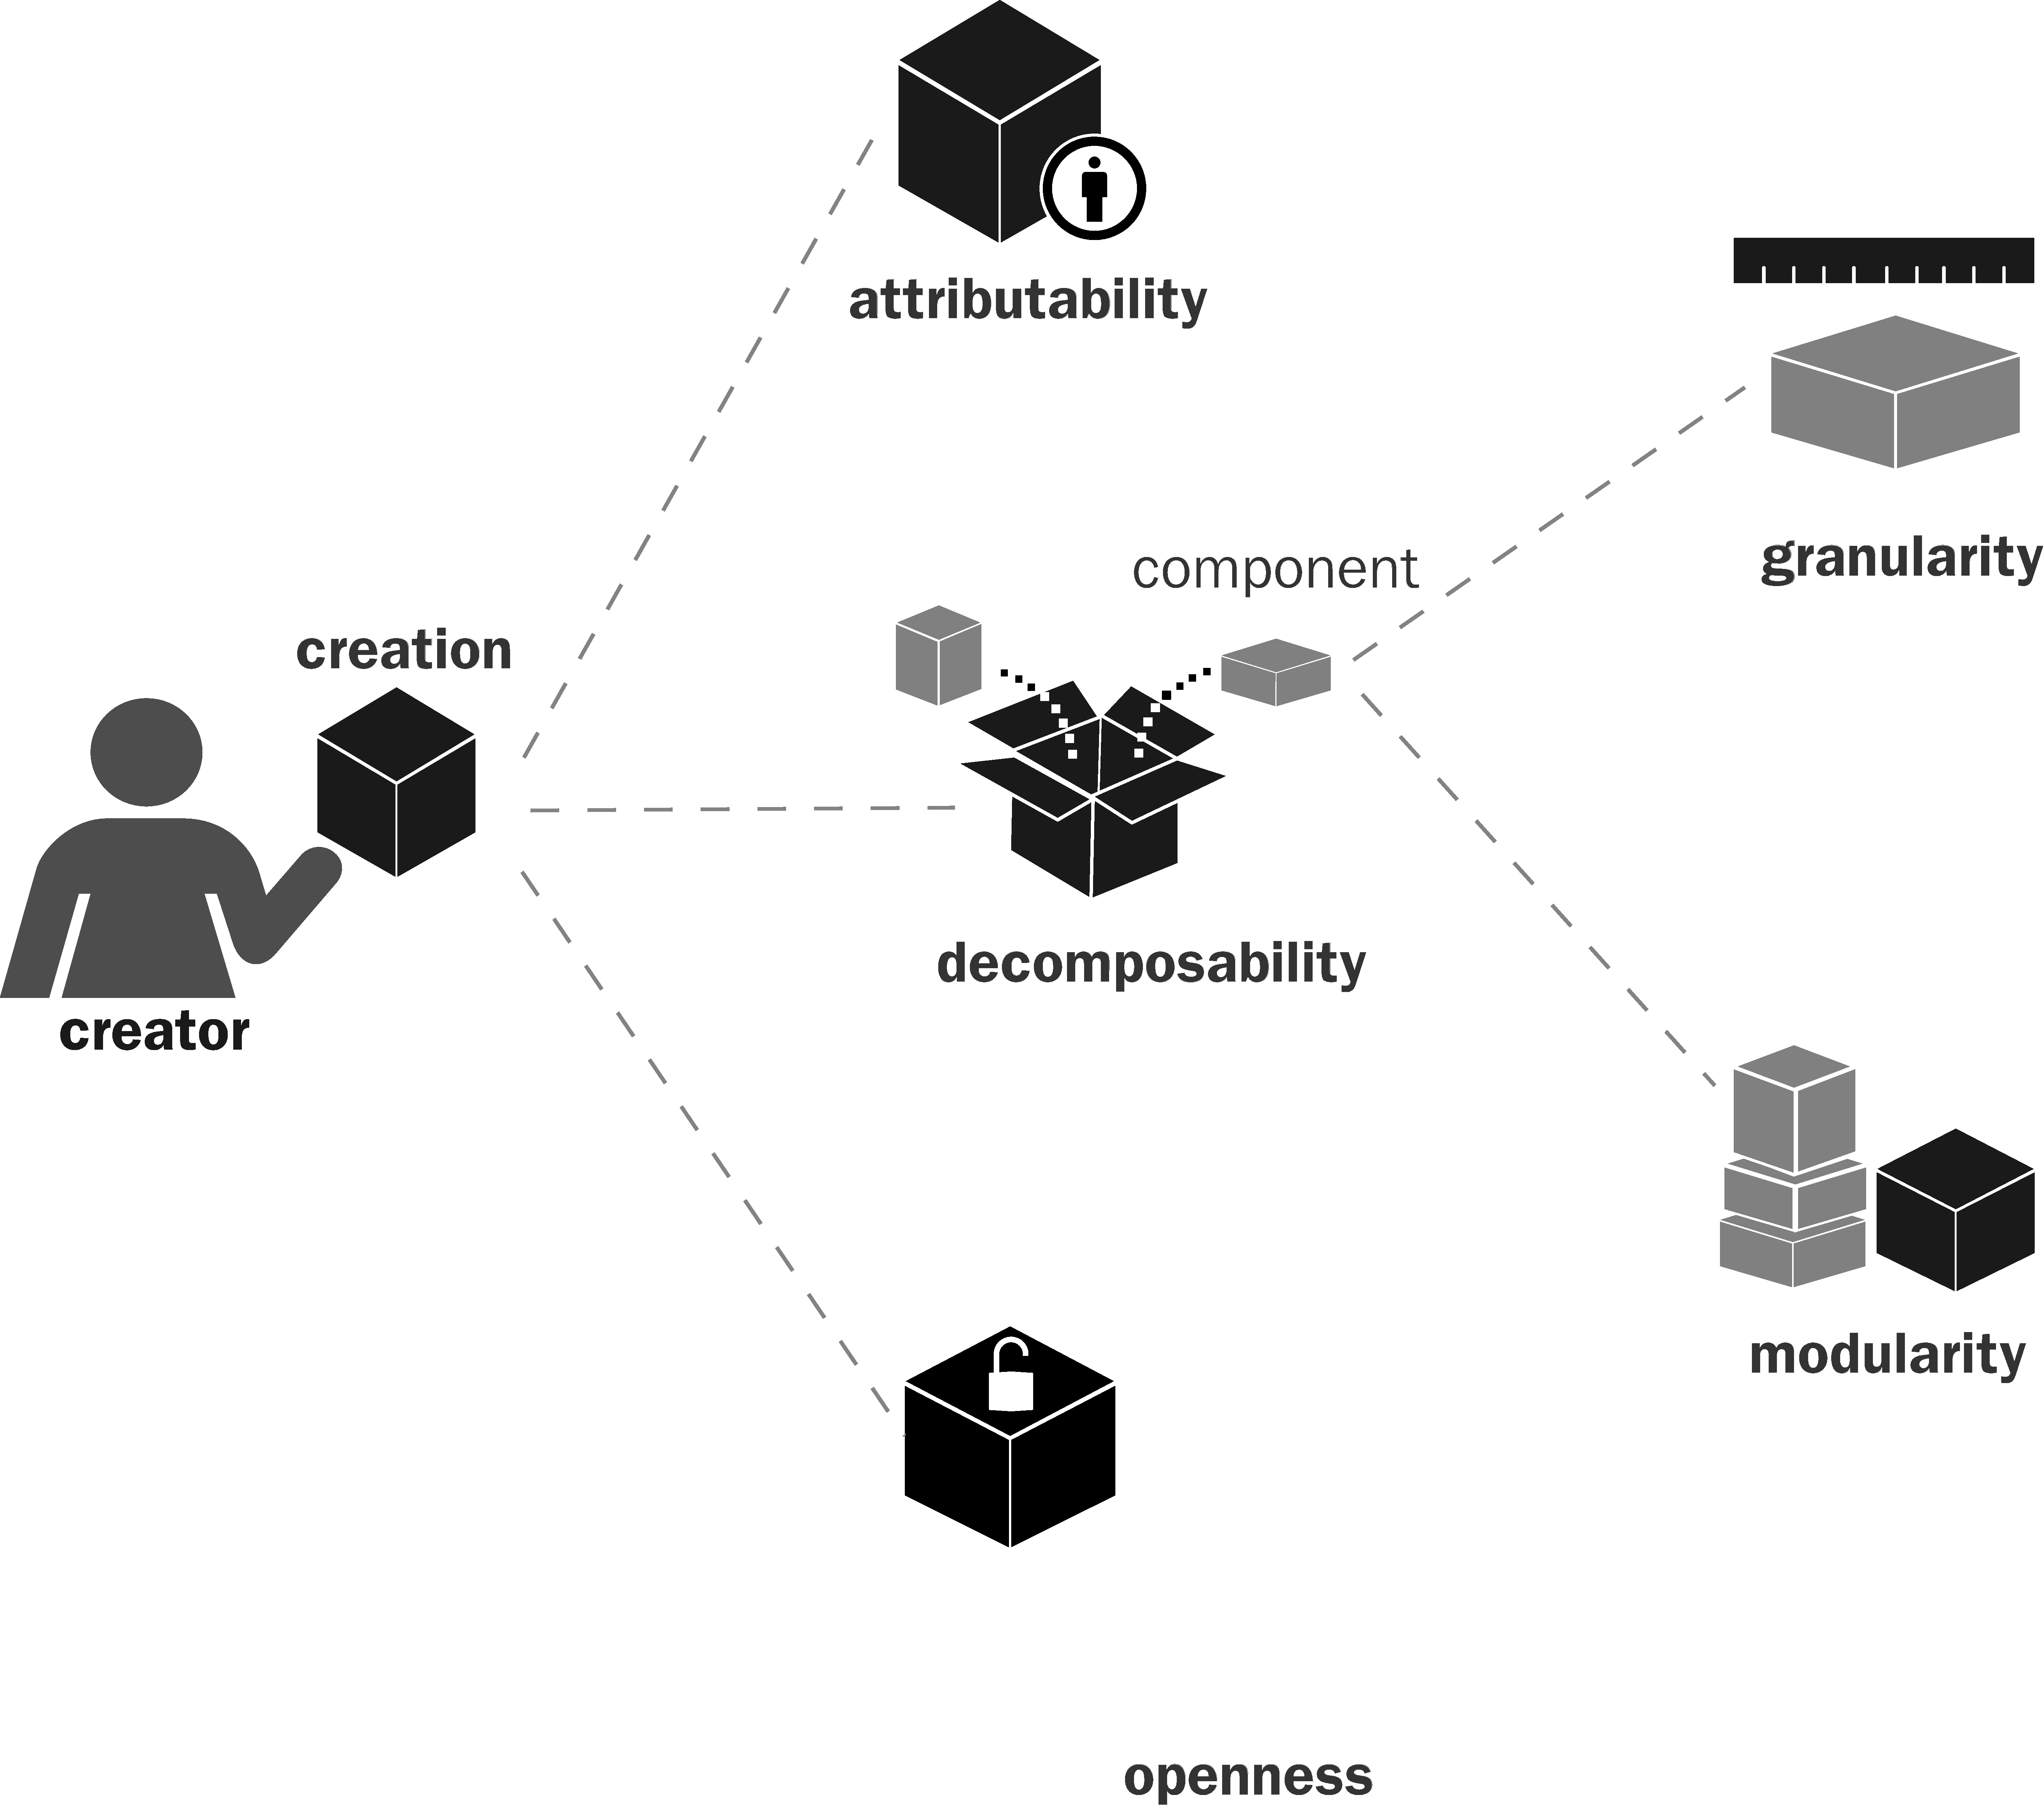
\includegraphics[width=3.25in]{figures/structure.pdf}
\caption{Structural dimensions of a remixing system (some icons taken from creativecommons.org, openclipart.org and thenounproject.com).}
\label{fig:structure}
\end{figure}

\subsubsection{Granularity}
Granularity is the size of project's modules \citep{benkler_coases_2002}. 
In Scratch, projects have several levels of granularity.
Projects are made of ``sprites'' such as characters in a game or elements in the user interface.
Each sprite can have ``scripts'' or stacks of programming blocks that control the sprite's behavior such as its position on the screen, its look, sound and interaction with other sprites and the user (by mouse, keyboard, or other sensors).
Each sprite also has one or more costumes or images that represent the various visual states of a sprite.
Sprites can also have sounds that are played programmatically; for example, a character in a game could make a sound each time it jumps.

\emph{Proposed Work.}
The Scratch Online Community, by default, only allows sharing at the coarsest degree of granularity: only projects can be shared. 
I plan to analyze the implications of this design decision and the ways  people get around the limitations of the architecure.

I have anecdotal evidence that Scratch participants get around the granularity limitations by sharing full projects with the sole intention of sharing a single sprite, script, image or sound.
This need for finer granularity often stems from a desire to engage in sharing practices that the original design did not anticipate. 
% mres: not the clearest example of fine granularity % For example, in previous work \citep{nickerson_appropriation_2011}, we have documented the existence of ``coloring contests'' where someone creates a project inviting others to add color to an image and then several other people do so by remixing the original project.
I plan to look at these practices in more detail to understand how a finer granularity mechanism would help support various types of creative and collaborative learning practices beyond the existing research that suggests that finer granularity is correlated with the number of people engaged in cooperative activities.

To analyze the effect of explicitly supporting finer degree of granularity through a natural experiment, I plan to analyze the adoption of ``Scratch Resources'' \footnote{Available at http://resources.scratchr.org}, a website created by members of the Scratch community to support sharing sprites, images and sounds. 
% TODO link to Von Hippel at al on user innovation

Some of my motivating questions are: 
How common is sharing and remixing across the various levels of granularity available (even if not explicitly supported)?
What are the types of participants and motivations for sharing finer grained components?
What role does granularity play in the likelihood of a project being remixed controlling for all other factors?
How do various levels of granularity affect the type and quality of remixes?
How do various levels of granularity support various levels of familiarity with Scratch -- are novices more likely to rely on coarser granularity when engaging in remixing as a scaffolding mechanism?

\subsubsection{Modularity}
\citet{benkler_coases_2002} defines modularity as the ``property of a project referring to the extent to which it can be broken down into smaller components, or modules, that can be independently and asynchronously produced before they are assembled into a whole.''
For this work, I separate two aspects of modularity:
1. The ease of \emph{integrating} such components into new creations or remixes.
2. The ease of \emph{decomposing} an existing project into smaller components, typically for remixing.
In this section I plan to analyze the term ``modularity'' by focusing on the first aspect.
In the next section, I focus on the second aspect under the term ``decomposability''.

\emph{Proposed Work.}
Some components or projects can be more easily integrated into new projects. 
One of the questions I am interested in exploring is what makes some components more modular than others.

For example, an image generated programmatically might be harder to integrate than one in bitmap format. 
A module that represents a cultural icon, such as Mario\footnote{Mario is a character in a popular video game called Mario Bros. from Nintendo Inc.}, is perhaps easier to integrate into other projects than an image of a less well-known character.
However, there are situations when new subcultural icons emerge within the Scratch community.
For example, a community member from New Zealand created a character called Maki-Tak. 
Maki-Tak became so popular in the community that other people started to create projects that included Maki-Tak itself of  that character or other characters inspired by it, often called Takis.
% Other examples: Mr Happy Man
Situations exist where some components are remixed despite their internal complexity, which might indicate that these could be built in a way that their internal complexity is hidden and remixing them is easy. 
For example there is a sprite created by an advanced Scratch user that represented a physics simulation of a string. 
This project was later remixed in a project where it represented a necklace.

I plan to operationalize the assessment of modularity by measuring its adoption through a number of remixes.
The assumption is that more modular components are remixed more.
I examine this in two types of components: the sample sprites, images and sounds that come with Scratch, and the ones that members of the community have created.
% Sample components are those that come preinstalled with Scratch. For example, sample images, sounds, sprites and occasionally projects.
% Community-generated are those created by end-users.
% The following paragraphs are commented out because mres mentioned that jetpack girl is not clear, plus I should make this research section shorter
%For example, ``jetpack girl'' is a sample sprite consisting of five costumes and  sounds for a flying character that can be controlled with the keyboard.
%The code of the sprite comes with an invitation to remix: ``Import me into your own project'' and an explanation on how to use it ``arrow keys make me fly''.
%These sample components are not only sprites, there are also hundreds of images and sounds that come with Scratch such as photographs of people, animals, things, and so on.
%Besides these sample components, there are thousands of components created by community members that are remixed and can be found in places like Scratch Resources and Scratch projects that explicitly state that they include sprites, images and sounds for others to reuse.

The type of questions I will to answer are:
1. What technical or cultural attributes are linked with component modularity? 
2. Are modular components used more often by newcomers, and do they provide scaffolding in their learning of Scratch programming?
3. Are community-generated components more often created by advanced users?

\subsubsection{Decomposability}
Building on the concept of modularity examined before, in this section I examine decomposability as the ease of decomposing a compiled project.
Decomposability is the ease of breaking something apart for remixing.
Therefore decomposability depends on the internal complexity of a project, which in itself depends on the expertise of the person attempting to decompose the project.
For example, one can argue that images in Flickr.com are harder to decompose than those in OpenClipart.org, which provides the source vectors, or Aviary.com which provides the bitmap images that were used to create an image.
The same happens with software applications that provide the source code in contrast with those that only provide the final compiled executable.
But even if the source code is provided, there are some cases where projects are ``impenetrable'' because of their complexity or a mismatch between the expertise of the person trying to decompose a project and the complexity of the project. 
For example, for a novice programmer having access to the source code of the Linux kernel might not allow for easy decomposability.

In Scratch, all the sources of a project are provided so the decomposability of a project depends, among other things, more on how interconnected its various components are. 
For example, sometimes sprites ``broadcast'' messages back and forth making their decomposability much harder than those that are self-contained.
Also some creators add instructions to their projects explaining how they can be broken apart, while others obfuscate their code to prevent remixing.

\emph{Proposed Work.}
I first do a manual analysis of a sample of projects to observe patterns of decomposability. 
Using the findings of this analysis I devise mechanisms to automate the evaluation of decomposability. 
For example, a decomposability metric could depend on the use of particular blocks (the ``broadcast'' block could reduce its ranking, while comments in the code would increase it), explicit obfuscation or matching between the typical expertise level of community members and the expertise required to understand a project.

I also look at remixes to analyze how different they are from their original project. 
The assumption would be that ``impenetrable'' projects would be correlated with no remixing or to superficial remixes, such as slight changes in the images, while highly decomposable projects are associated with significant differences between the remix and the original.

I also analyze the practices of code obfuscation and the strategies people use to discourage decomposability of their projects.

\subsubsection{Attributability}
Creators often want to get credit for their work. 
For example, the Creative Commons license originally had attribution as one of the options of their licenses, but after analyzing several years of usage of the licenses they found that few people waived the attribution clause. 
This led them to include attribution by default in all their licenses (and create a separate license for completely public domain works) \citep{brown_announcing_2004}.
To further our understanding of attribution when designing a remixing system it is important to know the role attribution plays in supporting cooperative behavior among members of a remixing online community.

In Scratch, we have run some design experiments playing with attribution. 
For example, we found evidence that suggests that about 20\% of creators object to seeing their projects remixed \citep{hill_responses_2010}.
We also have anecdotal evidence that people, who objected to remixing of their project, referred to a lack of credit as one of the problems.
To address this, I added a mechanism that would automatically give credit to the creator of the original project whenever a remix was uploaded (for example, ``Shared by John, based on Mary's project'').
Using that design intervention as a natural experiment, we found evidence that suggests people not only want to get credit but that they prefer the credit given by another person over the automatic attribution given by the system \cite{monroy-hernandez_computers_2011}. 

\emph{Proposed Work.}
I plan to extend this work with additional experiments.
For example, one of the common complaints against remixing is that the textual description of projects often gets copied from an original project onto its remixes.
This often gives the wrong impression that those notes were by the remixer rather than by the original creator.
I plan to add a mechanism to show a distinction between the notes by the originator and those added by the remixer.
These additional notes come with a mechanism to encourage remixers to explain how the original project was changed.
This will serve as a natural experiment to test the additional value of not only giving binary representation of attribution but also give a qualifier explanation to the connection between a remix and the original project.

% TODO: Other experiments: 
% - Creator endorsed attribution.
% - Diff

\subsubsection{Openness}
In this section I focus on analyzing a system's openness from the perspective of its norms and interactions with other systems.
The Scratch Online Community allows any of its members to download and remix any project, in that sense Scratch is more open than similar websites such as Kongregate.com or Newgrounds.com, which do not provide either the license, the environment, nor the technical features to freely open its content. 
The ethos of openness is present in Scratch through its terms of use, the license used by all projects shared, and the community moderation styled enforced by administrators.
However, this openness is not always understood or embraced by its members.
Also this openness is not always compatible with other systems.
For example, there are a some members of the community, who even after discussions with the administrators of the site, do not see enough value of openly sharing their work and decide to stop using the website. 
Additionally, there are other members of the community who encounter conflicts when remixing content from other online spaces that are not compatible with Scratch's openness. 
These conflicts often involve art-sharing websites like DeviantArt.com, from where Scratch creators sometimes get images for their projects.

\emph{Proposed Work.}
I plan to investigate the ways young people in Scratch embrace, understand and reject the way openness is interpreted in Scratch.
I try to examine whether young people see a value in openness and how a system is or is not able to surface these values through sociotechnical design.
I present a set of case studies that show the range of ways people embrace and reject openness and how the social and technical design of the website influence them. 

